%%%%%%%%%%%%%%%%%%%%%%%%%%%%%%%%%%%%%%%%%%%%%%%%%%%%%%%%%%%%%%%%%%%%%%%%%%%%%%%%
%2345678901234567890123456789012345678901234567890123456789012345678901234567890
%        1         2         3         4         5         6         7         8

\documentclass[letterpaper, 10 pt, conference]{ieeeconf}  % Comment this line out if you need a4paper

%\documentclass[a4paper, 10pt, conference]{ieeeconf}      % Use this line for a4 paper

\usepackage[ruled,vlined, linesnumbered]{algorithm2e}
\usepackage{graphicx}
\usepackage{caption}
\usepackage{siunitx}
\usepackage[utf8]{inputenc}
\usepackage{textcomp}

\SetAlFnt{\small}
\usepackage{algorithmic}
\algsetup{linenosize=\tiny}

\IEEEoverridecommandlockouts                              % This command is only needed if 
                                                          % you want to use the \thanks command

\overrideIEEEmargins                                      % Needed to meet printer requirements.

% See the \addtolength command later in the file to balance the column lengths
% on the last page of the document

% The following packages can be found on http:\\www.ctan.org
%\usepackage{graphics} % for pdf, bitmapped graphics files
%\usepackage{epsfig} % for postscript graphics files
%\usepackage{mathptmx} % assumes new font selection scheme installed
%\usepackage{times} % assumes new font selection scheme installed
%\usepackage{amsmath} % assumes amsmath package installed
%\usepackage{amssymb}  % assumes amsmath package installed

\title{\LARGE \bf
Exercise 1 - Explore \\
Intelligent Robotics \\
	\ \bf PENNY
}


\author{Federico Bacci, Daniel Clark, Laura Ferrante, Alessandro Pozzer, Saif Sidhik and Milan Mariya Tomy}


\begin{document}



\maketitle
\thispagestyle{empty}
\pagestyle{empty}


\begin{abstract}

This report introduces two different approaches for wheeled robot exploration in a constrained environment. Specifically, the algorithms were designed to complete the following task: \lq to maximize the floor space explored by the robot without crashing or getting stuck in one area\rq. After tuning the algorithms’ parameters, experimental data was gathered for each algorithm to compare their suitability for the task. The experimental results were analysed and compared to verify the performance of the algorithms, and then the more suitable algorithm was extended to better complete the task.

\end{abstract}

\section{Aims}
In developing each algorithm the initial aims were to prevent the robot from driving into obstacles or getting stuck in an area of the room. These conditions were considered a prerequisite for completing the final task of maximizing the space explored.

\section{Algorithms}
\subsection{Algorithm A}
The laser scanners angular range of 180\textdegree is split up into 7 sectors, 3 sectors on either side and a front sector in the center which is twice the size. The average distance read from each sector is compared with the detection distance constant, which the robot uses to decide whether to turn, or to go straight. After an obstacle is detected, the turn angle is decided by which sector detected the obstacle; the closer to the center sector it is, the greater the turn angle.

\subsection{Algorithm B}
The behaviour of this algorithm is such that when the robot detects an obstacle directly ahead of it, it rotates until the obstacle is no longer in front of it, then continues moving forward.

\subsubsection{Detection function}
When a block of 5 consecutive pieces (signifying a large enough object) of data in the front facing section of the scan arc are lower than detection distance constant, the robot stops and calls the turn function.

\subsubsection{Turn function}
The turn function averages the data on the left and right of the scan and uses whichever is greater to determine which direction to turn. The robot will rotate by a very small, fixed angle every time turn is called. 

\section{Characterisation}
Initially, the parameters were deduced from simple observations. A new set of parameters was then evolved from the initial parameters. For each set of parameters the robot was started in different areas of the floor in "more critical" locations (corners, chairs, etc). The number of crashes was collected after each test and the set of parameters which leads to fewer crashes was considered the new set.

\section{Hypothesis 1}
The first hypothesis is that algorithm A will be worse at avoiding obstacles than algorithm B. This is because it takes an average over a large area so may not notice a obstacle in its path. If this is the case, Algorithm B should be taken forward and developed further, if not, Algorithm A should be carried forward instead.
\subsection{Method}
The test will be run 5 times for each algorithm, each starting in the same place. The robot will be placed in position A4, facing towards B4, as seen in Fig. \ref{fig:map}. 
The robot will be switched on and algorithm A will be started along with a timer.
If a crash occurs, the time from the timer will be noted, the robot will be moved slightly so that it is 50cm from the nearest obstacle, and both the robot and the time shall be restarted.
\begin{figure}[b]
\centering
\captionsetup{justification=centering}
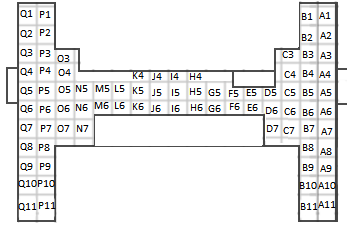
\includegraphics[scale=0.68]{maplgfloor}
\caption{The Grid Layout Of The CS Lower Ground Floor}
\label{fig:map}
\end{figure}
\begin{figure}[tb]
\centering
\captionsetup{justification=centering}
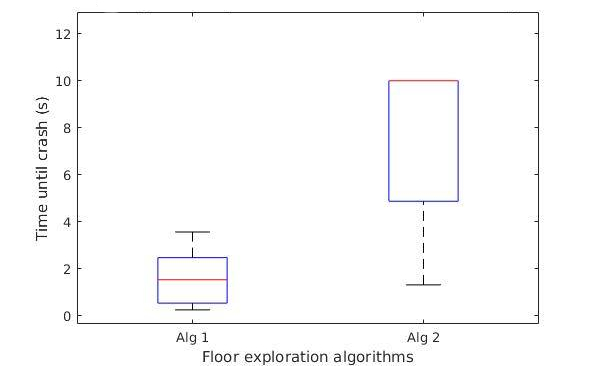
\includegraphics[scale=0.4]{box_plot}
\caption{A Graph To Compare The Times Taken Before Crashing For Algorithms A And B}
\label{fig:boxplot}
\end{figure}
\subsection{Results and Analysis}
The data gathered from the tests for hypothesis 1 are presented in Fig. \ref{fig:boxplot}. All attempts which did not crash in the 10 minute period were given a time of 10 minutes to enable the data to be graphed.

From the data and graphs drawn of the first test it is evident that algorithm B was better suited to the task of avoiding obstacles. It can be seen that almost all the test runs for algorithm A crash before the runs of algorithm B. It is also noteworthy that most runs from the algorithm B tests did not crash at all in the 10 minute period.

The t-test was performed with a null hypothesis that the average of the times until a crash is the same for algorithms A and B and a confidence at 95\%. The p-value is 0.001 which is extremely statistically significant. This p-value shows that we are able to reject the null hypothesis and proves that B is more suitable than A.

\section{Improvements}
Based on the analysis of the hypothesis 1 results, it was decided that algorithm B should be taken forward and developed such that it could better explore the environment.

\subsection{Algorithm C}
Algorithm C is the same as algorithm B, except with the following addition to the detection algorithm.
\begin{algorithm}
	
	\KwIn{ Data from the sensor $S$. Let $m$ be the minimum size of an obstacle, $h$ the size of the detected obstacle, $\theta$ the angle }
	
	\If{obstacle is not close to the robot}{
		\If{mean(extreme left side of S) $> d_1$ $\land$ mean(extreme right side of S) $> d_1$}{
			\If{mean(right side of S) $> d_2$ $\land$ mean(left side of S) $> d_2$}{
				turn right
				}
			\If{mean(right side of S) $> d_2$ $\vee$ mean(left side of S) $> d_2$}{difference = mean(right side of S) - mean(left side of S) \\
				\If{difference $>= 0$}{turn right}
				\Else{turn left}}
			}	
		
	}	
	
\end{algorithm}

\section{Hypothesis 2}
The second hypothesis is that algorithm C will explore more of the floor space than algorithm B. Algorithm C takes into consideration the distance detected by the robot even when there is no object directly in front of it, to decide its angle and direction of rotation. Hence it tends to cover more area while exploring, which would make algorithm C explore more space than algorithm B.

\subsection{Method} 
The tests will be conducted by splitting the environment into squares of \SI{1.5}{m^2} for calculating the area explored by the robot.  The robot will be placed at square A4, facing B4. Both algorithms B and C will be run on the robot and the robots movements across the grid will be monitored for 10 minutes in each case. The squares that the robot crosses will be noted down. For each algorithm, five sets of tests will be conducted.
For each algorithm and for every square, the percentage of tests for which the robot crossed a particular square was calculated.

\begin{figure}[t]. 
\centering
\captionsetup{justification=centering}
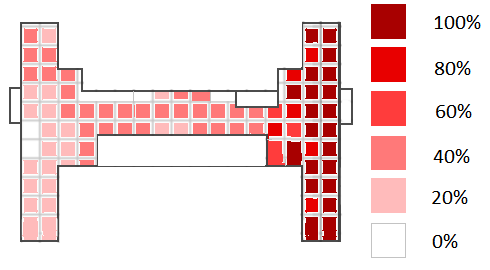
\includegraphics[scale=0.4]{maplgfloor3_superbasic}
\caption{The Percentage Of Tests For Which The Robot Crossed Each Square When Using Algorithm B}
\label{fig:superbasicfloor}
\end{figure}

\begin{figure}[t]
\centering
\captionsetup{justification=centering}
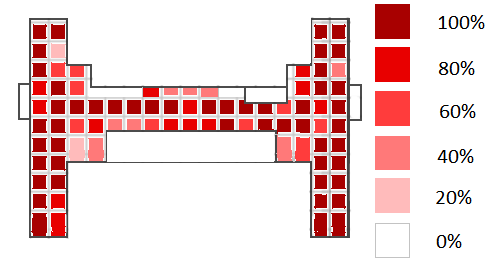
\includegraphics[scale=0.4]{maplgfloor3_superbasicopenspace}
\caption{The Percentage Of Tests For Which The Robot Crossed Each Square When Using Algorithm C}
\label{fig:superbasicopenspacefloor}
\end{figure}
\subsection{Results and Analysis}
It is very evident from the two figures Fig. \ref{fig:superbasicfloor} and Fig. \ref{fig:superbasicopenspacefloor} that a significantly increased number of squares were entered by algorithm C, and so the improvements made to algorithm B work well.

The t-test was performed with a null hypothesis that the number of explored squares is the same for algorithms B and C. The level of confidence was set at 95\%. 0.001 was found to be the p-value, which is extremely statistically significant. This p-value shows that we are able to reject the null hypothesis and proves that C is more suitable than B.

\section{Conclusions}

A final test was run to measure how long it took algorithm C to crash, the test was extended past the 10 minute limit and did not crash until a time of 28 minutes.

We can see from the analyses that algorithm C successfully explorers the environment with a very low chance of crashing into either stationary or mobile objects.


\end{document}
